\begin{figure}[tb]
\centering
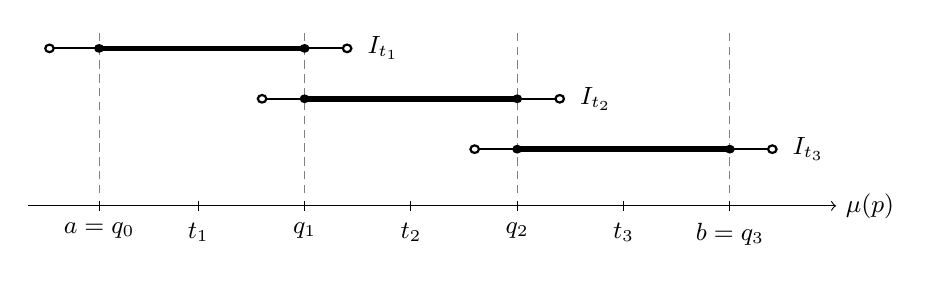
\begin{tikzpicture}[x=0.9cm,y=0.8cm,font=\small]
  \draw[->,thin] (-0.4,0) -- (11.0,0) node[right] {$\mu(p)$};
  \foreach \x/\label in {0.6/{a=q_0},2/{t_1},3.5/{q_1},5/{t_2},6.5/{q_2},8/{t_3},9.5/{b=q_3}} {
    \draw (\x,0.08) -- (\x,-0.08);
    \node[below] at (\x,-0.12) {$\label$};
  }
  \foreach \x in {0.6,3.5,6.5,9.5} {
    \draw[gray,densely dashed,thin] (\x,0.2) -- (\x,2.75);
  }
  \draw[thick] (-0.1,2.5) -- (4.1,2.5);
  \draw[fill=white,thick] (-0.1,2.5) circle (0.06);
  \draw[fill=white,thick] (4.1,2.5) circle (0.06);
  \draw[line width=2pt] (0.6,2.5) -- (3.5,2.5);
  \fill (0.6,2.5) circle (0.07);
  \fill (3.5,2.5) circle (0.07);
  \node[right] at (4.25,2.5) {$I_{t_1}$};
  \draw[thick] (2.9,1.7) -- (7.1,1.7);
  \draw[fill=white,thick] (2.9,1.7) circle (0.06);
  \draw[fill=white,thick] (7.1,1.7) circle (0.06);
  \draw[line width=2pt] (3.5,1.7) -- (6.5,1.7);
  \fill (3.5,1.7) circle (0.07);
  \fill (6.5,1.7) circle (0.07);
  \node[right] at (7.25,1.7) {$I_{t_2}$};
  \draw[thick] (5.9,0.9) -- (10.1,0.9);
  \draw[fill=white,thick] (5.9,0.9) circle (0.06);
  \draw[fill=white,thick] (10.1,0.9) circle (0.06);
  \draw[line width=2pt] (6.5,0.9) -- (9.5,0.9);
  \fill (6.5,0.9) circle (0.07);
  \fill (9.5,0.9) circle (0.07);
  \node[right] at (10.25,0.9) {$I_{t_3}$};
\end{tikzpicture}
\caption{Combining three local families, schematically. Each thick closed
interval $[q_{j-1},q_j]$ lies inside the open neighborhood $I_{t_j}$
where its family is valid. The shifts in \eqref{eq:affine-shifts} force
the limiting minimum exponent of an active label into this closed
interval. At a cut, either neighboring family remains valid.}
\label{fig:intervals}
\end{figure}
